\documentclass[a4paper,UTF8]{article}
\usepackage{ctex}
\usepackage[margin=1.25in]{geometry}
\usepackage{color}
\usepackage{graphicx}
\usepackage{amssymb}
\usepackage{amsmath}
\usepackage{amsthm}
\usepackage{booktabs}
\usepackage{caption}
\usepackage{fancyhdr}
\usepackage{extramarks}
\usepackage{amsfonts}
\usepackage{tikz}
\usetikzlibrary{arrows}
\usepackage{algorithm}
\usepackage{algorithmicx}
\usepackage{algpseudocode}
\usepackage{listings}

%\usepackage[thmmarks, amsmath, thref]{ntheorem}
\theoremstyle{definition}
\newtheorem*{solution}{Solution}
\newtheorem*{prove}{Proof}
\usepackage{multirow}

%
% Basic Document Settings
%

\topmargin=-0.45in
\evensidemargin=0in
\oddsidemargin=0in
\textwidth=6.5in
\textheight=9.0in
\headsep=0.25in

\linespread{1.1}

\pagestyle{fancy}
\lhead{\hmwkTitle}
\chead{\hmwkClass\ (\hmwkClassInstructor\ \hmwkClassTime)}
\rhead{\hmwkAuthorName}
\lfoot{\lastxmark}
\cfoot{\thepage}

\renewcommand\headrulewidth{0.4pt}
\renewcommand\footrulewidth{0.4pt}

%
% Homework Details
%   - Title
%   - Due date
%   - Class
%   - Section/Time
%   - Instructor
%   - Author
%

\newcommand{\hmwkTitle}{Assignment \ \#1}
\newcommand{\hmwkDueDate}{September 12, 2017}
\newcommand{\hmwkClass}{Problem Solving}
\newcommand{\hmwkClassTime}{}
\newcommand{\hmwkClassInstructor}{Professor Chen}
\newcommand{\hmwkAuthorName}{李志琦 161220074}

%--

%--
\begin{document}

\section*{Chapter 24 }

\subsection*{24.1-2}
\begin{itemize}

  \item if there is a path from $s$ to $v$ then: \\
  there must be a shortest-path between s and v, so we can assume the path\\
  has k edges, so the path is: $s \to v_0 \to v_1 \ldots v_{k-3} \to v$ \\
  from \textbf{\textit{Lemma 24.2}}  we know $v.d= \delta (s.v)$\\
  so $v.d=w(s,v_0)+w(v_0,v_1)+\ldots+w(v_{k-3},s)<\infty$\\
  \item if \textbf{Bellman-Ford} terminates with $v.d<\infty$ then:\\
  we get that the vertice $v$ is relaxed, we can easily get that if a vertice\\
  can be relaxed, so:
  \[
   v.d\le \delta(s'.u)+w(s',v)
   \]
  so $s'$ can be reached from s, and $s'$ has edges with v, so there is a path between s and v.
\end{itemize}
\subsection*{24.1-3}
\begin{algorithm}[h]
  \caption{Bellman-Ford($G$,$w$,$s$)}
  \begin{algorithmic}[1]
    \State INITIALIZE-SINGLE-SOURCE($G$,$S$)
    \State copy each vertice's $d$ to a array $COPY[|G.V|]$
    \For{$i=1$ to $|G.v-1|$}
      \For{each edge $\in G.v$}
      \State RELAX($u,v,w$)
      \EndFor
      \State compare the latest vertice's $d$ to the old one in $COPY$ array, if nothing changed, we make it and break.
    \EndFor
    \For {each edge $(u,v) \in G.E$ }
    \If {$v.d>u.d+w(u,v)$}
    \Return FALSE
    \EndIf
    \EndFor

  \end{algorithmic}
\end{algorithm}

\subsection*{24.1-4}
.\\
we only need to change $return \ FALSE$ to $v.d=-\infty$ in line 7\\
because if vertice $v$ iS the vertice we want to find, and we assume
the vertice $u$ is also in the path including negative-weight cycles
 we know before each $REALX(u,v)$ , v.d will be larger than $u.d+w(u.v)$
 so only vertices like $v$ can match the $line 6$ 's condition.

\subsection*{24.2-2}
.\\
because the last vertice's adjance list is empty, it doesn't matter
if the last loop does or not, because no more RELAX func will be called

\subsection*{24.3-2}
.\\
in proof, we get $\delta(s,y)\le\delta(s.u)$, but when there are negative-weight
path, $\delta(s,y)\le\delta(s.u)$ will not be true always. it can easily get when
there is a negative-wight edge from $u$ to $y$


\subsection*{24.3-4}
\begin{itemize}
  \item first, $s.d=0 s.\pi=NIL$
  \item for any vertice, if its $\pi$ is NIL, its $d$ should be $+\infty$
\end{itemize}
\begin{algorithm}[h]
  \caption{Check-Bellman-Ford($G$,$w$,$s$)}
  \begin{algorithmic}[1]
    \For { each vertice $v \in G.v$}
      \For { each edge $u \in G.adj[v]$}
        \If{$v.d>u.d+w(u.v)$}
          \Return False
        \EndIf
    \EndFor
    \EndFor

  \end{algorithmic}
\end{algorithm}

 \subsection*{24.3-7}
.\\
 the num of edges $edges = \sum_{(u,v)\in E} w(u,v)-1$ \\
 the num of vertices $vertices = edges-1  $

 \subsection*{24.5-2}
 .\\
 let vertice $s,u,v$ be the three vertices of a triangle,and the weight of
 $(u,v),(s,u),(s,v)$ are 2,2,0\\
 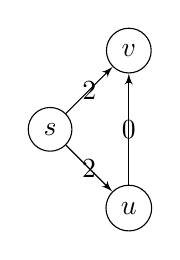
\begin{tikzpicture}
 \tikzset{vertex/.style = {shape=circle,draw,minimum size=0.5em}}
 \tikzset{edge/.style = {->,> = latex'}}
 % vertices
 \node[vertex] (s) at  (0,1) {$s$};
 \node[vertex] (u) at  (1,0) {$u$};
 \node[vertex] (v) at  (1,2) {$v$};

 %edges
 \draw [edge] (s) to  node {2} (u);
 \draw[edge] (s) to  node {2} (v);
 \draw[edge] (u) to  node {0}(v);
 \end{tikzpicture}
 \subsection*{24.5-5}
.\\
the result we want get is like this \\
$$v.\pi =v_1, v_1.\pi=v_2,\ldots ,v_n.\pi=v$$
to simplify, we can let $v.\pi=u, u.\pi=v$
so  the graphy in $24.5-2$ can match it, there is a shortest
path to $v$ is $s\to u \to v$, and also a shortest path to $u$ is
$s\to v \to u$, so let $v.\pi=u, u.\pi=v$, we make it.


\subsection*{24.2}

\subsubsection*{a}
.\\
assume that box $a(a_1,a_2,\ldots,a_d)$ nests within box $b(b_1,b_2,\ldots,b_d)$, and box $c(c_1,c_2,\dots,c_d)$ nests within box $c$
so there is permution $\pi$ on $\{1,2,\ldots,d\}$,such that:
$$a_{\pi(1)}<b_1,a_{\pi(2)}<b_2,\ldots,a_{\pi(d)}<b_d$$
$$b_{\pi(1)}<c_1,b_{\pi(2)}<c_2,\ldots,b_{\pi(d)}<c_d$$
let the above two sets be two func $f$ and $g$,we can easily get a new func $h=f(g)$
beause both are bijection.
we can get  $$a_{\pi(1)}<c_1,a_{\pi(2)}<c_2,\ldots,a_{\pi(d)}<c_d$$
so nesting relation is transitive.
\subsubsection*{b}
.\\
sort both two dimensition  from small to large, then
let $boolean a = x_i>y_i for i in range(1,d+1)$
after the a be initialized, and if its value changes, then one can not nests within another
total time is $O(d\log d)$

\subsubsection*{c}
.\\
we can first sort all n box's dimensition. which is $O(nd\log d)$,
we let each box be a vertice in a graphand then for each pair vertices $u,v$ in $G.V$
first we should find if there is path from $u$ to $v$, if it is, that menas $u$ can be nests within $v$
else to check if one box can nest within another,if $u$ can nest within $v$ so add a arrow from $u$ to $v$.
at last find the longest path in G.\\
the running time is $O(nd(\log d+n))$


\subsection*{24.3}
\subsubsection*{a}
.\\
I refer to the answer on the website,the main idea is tranforming the formula
$$R[i_1,i_2]\cdot R[i_2,i_3]\ldots R[i_k,i-1]>1$$
to
$$-\ln(R[i_1,i_2])-\ln(R[i_2,i_3])\ldots -\ln(R[i_k,i_1])<0$$
so we kan use Bellman Ford algorithm to detect if exists.
when BF returns FALSE, it exists
\subsubsection*{a}
.\\
when BF return FALSE, which vertice gose wrong?\\
the vertice $v$ is the one whose $d$ will be relaxed in $|V|_{th}$ loop in the code, but
unfortunately we only have $|V|-1$ loop, so we can change Bellman Ford algorithm
let it has $|2×V|-1$ loop but after $|V|-1$ loop we will check and we will save the vertice
that cause FALSE and not return,and let its predecessor be $u$, all the vertices we save are the vertices on the nagetive-weight cycles.
so we can get the cycle by these vertices and their predecessor\\

\end{document}
